\section{Challenges}\label{challenge}
To be honest, UFO data is really difficult to process and analyze. There are limited number of reports, and it's difficult to find out suitable models along with correct labels to predict. Actually we have tried many other ways, all of which finally failed to achieve satisfactory results.

\begin{figure}[H]
    \centering
    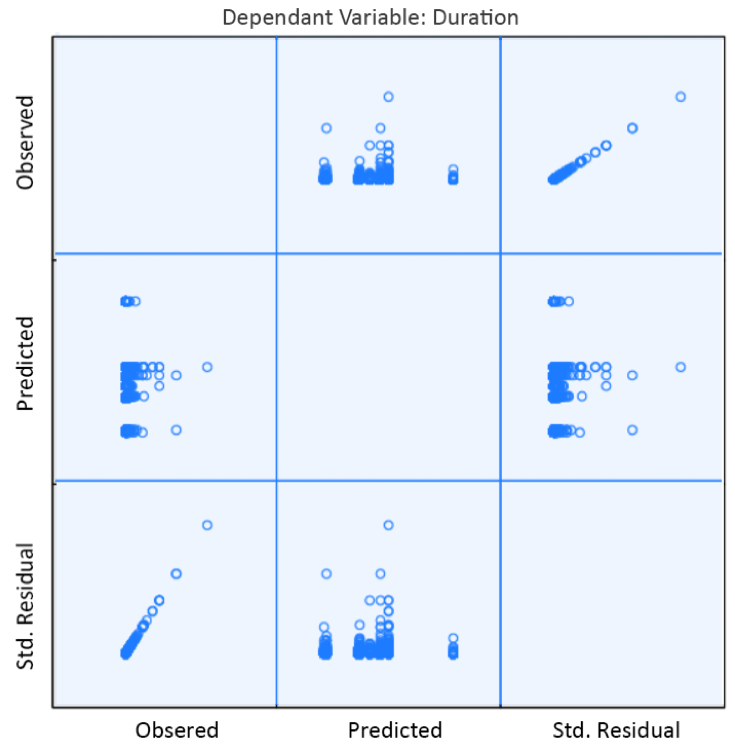
\includegraphics[width=7cm]{figure/correlation.png}
    \caption{intercept + weather}
    \label{correlation}
\end{figure}

At first, we try to predict duration, shape or location based on other features. However, when we do statistic analysis on a variety of meteorological features (temperature, wind speed, humidity, visibility, etc.,), geographical features along with the UFO reports data, most of them do not have significant correlations with other features of UFO reports data. For example, figure \ref{correlation} indicates the weak correlation between other features and duration of UFO appearances.

We have tried a lot of machine learning algorithms to detect fake reports. One approach is unsupervised learning --- clustering true and fake reports. However, as our training result shows, the internal cluster measures~\cite{clustermeasure} are not good, actually only 0.2 out of 1.~\footnote{$ 1 - \frac{compactness}{separation} $} Another way is to convert a classification problem on imbalanced data to an outlier detection problem only on positive data. We use one-class SVM to model true reports only. Based on true report boundary gained above, we use this model to detect which report is outlier,i.e., out of boundary. However, this method only generates a detecting accuracy slightly greater than 50\%, which is absolutely unacceptable.